\documentclass[a4paper,utf8]{article}
\usepackage[heading,fancyhdr]{ctex}
\usepackage{amsmath,amssymb,geometry,lastpage,ulem}
\usepackage{array,tabularx}
\usepackage{siunitx}
\usepackage{graphicx,floatrow}
\lineskiplimit=1pt
\lineskip=3pt
\geometry{
    top=25.4mm, 
    left=25mm, 
    right=25mm, 
    bottom=25mm,
    headsep=5.9mm,
}
\ctexset{
    section = {format+=\raggedright}
}
\newcommand{\fgref}[1]{图~\ref{#1} }
\newcommand{\seqref}[1]{式~(\ref{#1})}
\pagestyle{fancy}
\fancyhf{} \fancyhead[C]{材料科学基础实验} \fancyfoot[C]{\thepage\;/\;\pageref{LastPage}}
\begin{document}
\begin{center}
    {\mbox{}\\[7em]\zihao{2}\bfseries\songti%
    材料科学基础实验预习报告}\\[34mm]
    {\zihao{-3}\bfseries\songti
    实验名称:\uline{\hfill\mbox{四探针法测量半导体电阻率和薄层电阻}\hfill} \\[2.9mm]
    学\quad 号:\uline{\makebox[25mm]{22301070}}\hfill
    姓\quad 名:\uline{\makebox[25mm]{杨雨燃}}\hfill
    班\quad 级:\uline{\makebox[25mm]{22材物}} \\[2.9mm]
    合作者:\uline{\makebox[25mm]{}}\enspace~
    桌\quad 号:\uline{\makebox[25mm]{}}\hfill\mbox{}\\[2.9mm]
    指导教师:\uline{\makebox[30mm]{艾斌}}\hfill\mbox{} \\[2.9mm]
    实验日期:\uline{\makebox[30mm]{}}\hfill\mbox{} \\[58.7mm]
    {\zihao{4}\bfseries\songti
    实验考核\\[3mm]
    \extrarowheight=3mm
    \begin{tabularx}{150mm}{|X|X|X|X|X|}\hline
        \hfil 项目 \hfil  & \hfil 实验预习 \hfil & \hfil 实验过程 \hfil & \hfil 分析与讨论 \hfil & \hfil 总评 \hfil \\[3mm] \hline
        \hfil 评价 \hfil &  &  &  &  \\[3mm] \hline
    \end{tabularx}
    }
    }
\end{center}
\newpage
\section*{【实验目的】}
    \begin{enumerate}
        \item 理解四探针方法测量半导体电阻率和薄层电阻的原理;
        \item 学会用四探针方法测量半导体电阻率和薄层电阻;
        \item 针对不同几何尺寸的样品,了解其修正方法;
        \item 了解影响测量结果准确性的因素及避免方法
    \end{enumerate}
\section*{【实验原理】}%简单描述,含必要的公式和附图;
    \subsection{半导体材料体电阻率的测量}
        \subsubsection{半无穷大样品体电阻率的测量}
            
            在四探针法中,当电流 $I$ 通过探针以点电流源形式注入半导体材料内部时,电流密度在材料内部是均匀分布的,具体是以探针尖为球心沿径向放射状分布。四根金属探针排成一列,间距均为 $S$。在这种情况下,当探针 1 和探针 4 通以电流 $I$ 时(探针 1 为正极,探针 4 为负极),探针 2 和探针 3 上测得的电压为 $V_{23}$。只要样品厚度及边缘与探针的最近距离大于四倍探针间距,半无穷大样品的体电阻率 $\rho$ 可以表示为:            \begin{equation*}
                \rho = 2\pi S\cdot\frac{V_{23}}{I} \label{eq:0}
            \end{equation*} 
            
            式中$\rho $以cm为单位,而所测电压,电流分别以mV,mA为单位。此外本实验测量时的探针间距S =0.1cm相比于样品的尺寸符合上式使用的要求,将电流I选取为2$ \pi $S =0.628 mA时,2,3探针所测电压示数即为所测电阻率的示数(直读法)。
            
            半导体材料的电阻率对温度比较灵敏,因此,测试半导体材料的电阻率时不但要记录测试的环境温度,还要将该温度下的实测电阻率修正到 23℃下的电阻率,引入修正系数 $F_T$ : 
            \begin{equation*}
                \rho =\frac{2\pi S}{F_T}\cdot\frac{V_{23}}{I}
            \end{equation*}
        \subsubsection{无穷大薄样品体电阻率的测量}
        无穷大薄样品是指厚度 d 小于探针间距 S 而横向尺寸无穷大的样品。根据无穷大样品的模型推导,电流I以点接触的形式进入样品,此时形成的电流密度呈柱对称分布,取距离点电源 1 米处的电势为零,
        用类似半无穷大样品的方法,等间距一字排开的四根金属探针压在薄样品表面,故无穷大薄样品的电阻率 $\rho$ 可表示为:
            \begin{equation*}
                \rho =\frac{\pi V_{23}}{I \ln 2} \label{eq:1}
            \end{equation*}

        电压电流分别以mV,mA为单位。
    \subsection{半导体材料电阻的测量}        
        \subsubsection{半导体薄层电阻(或方块电阻)的测量}
        四探针法除了可以测量硅片、硅锭等体材料的电阻率外,还可用来测量扩散层、绝缘衬底上的半导体薄膜的薄层电阻。薄层电阻又称为方块电阻,是指平行于电流方向的正方形表面下的半导体薄层在电流方向上的电阻。
        如果扩散片的结深用 $X_j$ 表示,根据定义,方块电阻 $R_{sq}$ 可表示为:
            \begin{equation*}
                R_{sq}=\rho\frac{L}{L\cdot X_{j}}=\frac{\rho}{X_{j}} \label{eq:2}
            \end{equation*}
            将其视为无穷大薄样品,可得其电阻表示为
            \begin{equation*}
                R_{sq}=4.5324\frac{V_{23} d}{I} \label{eq:3}
            \end{equation*}
            实际测量中,只要薄层的厚度小于 $0.5S$,并且样品面积相对于探针间距 $S$ 可视为无穷大时,就可以利用上式计算薄层电阻。如果不能将样品的横向面积视为无穷大,也需要使用包含修正因子 $F$ 的公式来计算方块电阻:
            \begin{equation*}
                R_{sq}= F \frac{V_{23}}{I} \label{eq:4}
            \end{equation*}

            由上式可知,如果半导体薄层可以视作无穷大薄样品,可以把测试电流设为 4.5324 mA,然后从电压表上直接读出样品的方块电阻。
        
\section*{【实验仪器】}%规格及参数
    KDY-1 型四探针电阻率/方阻测试仪,一台计算机;p 型单晶硅棒(电阻率样品)、p 型单晶硅片(薄样品)、p 型硅基底上的 n 型扩散片(薄层电阻样品)各一个
    \section*{【实验过程】}
    \subsection*{测量样品电阻率或方块电阻的操作步骤}
    \begin{enumerate}
        \item 打开 KDB-1 四探针测试仪后面板上的电源开关,将“电阻率/方块电阻测试切换开关”($\rho/R$ 开关)设置到相应位置。
        \item 将样品置于样品台上,调节探针使其落在样品的测试点,注意轻压探针避免损坏。
        \item 调节测试电流和恒流源电压档位,使得电压表显示稳定的测试电流和电压值。
        \item 记录测试电流和电压,计算样品的电阻率或方块电阻,完成测量后取走样品。
    \end{enumerate}
    
    \subsection*{测量 p 型硅棒的电阻率}
    使用推荐的测试电流对硅棒横截面上多个位置处的电阻率进行测量,记录结果并修正至 \SI{23}{\degreeCelsius}。利用公式计算电阻率分布的不均匀度。
    
    \subsection*{测量 p 型单晶硅片(薄样品)的电阻率}
    \begin{enumerate}
        \item 直接读取电流和电压,计算硅片的电阻率。
        \item 根据测得的电流和电压,以及硅片的尺寸,计算电阻率并修正至 \SI{23}{\degreeCelsius}。
    \end{enumerate}
    
    \subsection*{测量 p 型单晶硅衬底上的 n 型扩散片的方块电阻}
    在扩散片中心位置进行方块电阻的测量,记录结果并修正至 \SI{23}{\degreeCelsius}。
    
    \subsection*{测量 p 型单晶硅衬底上的 n 型透明导电玻璃的方块电阻}
    测试方法与要求与扩散片一致。

\section*{【实验数据】}
    制作了excel表格,附后
    \begin{figure}[!ht]
        \begin{floatrow}
            \ffigbox[80mm]{\caption{表格截图1}}{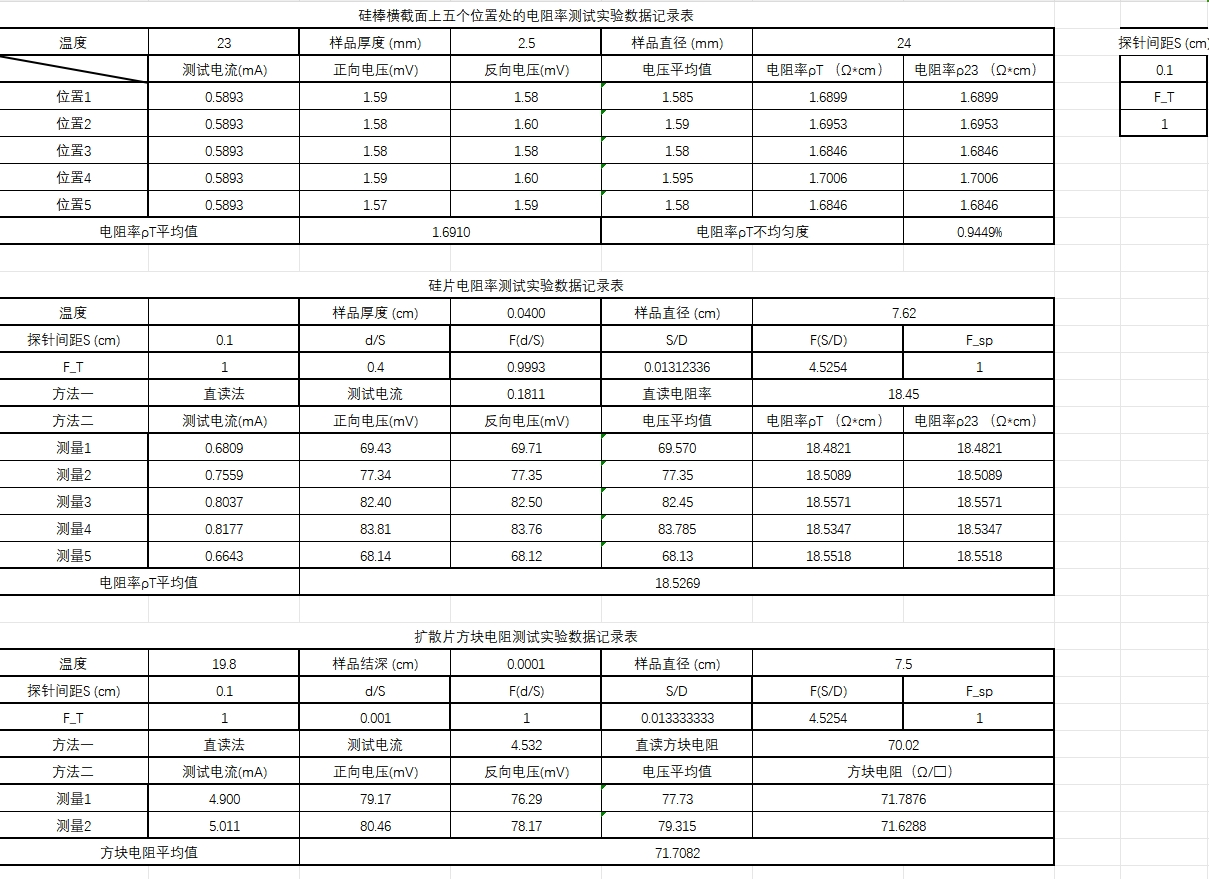
\includegraphics[width=80mm]{1.png}}
            \ffigbox[80mm]{\caption{表格截图2}}{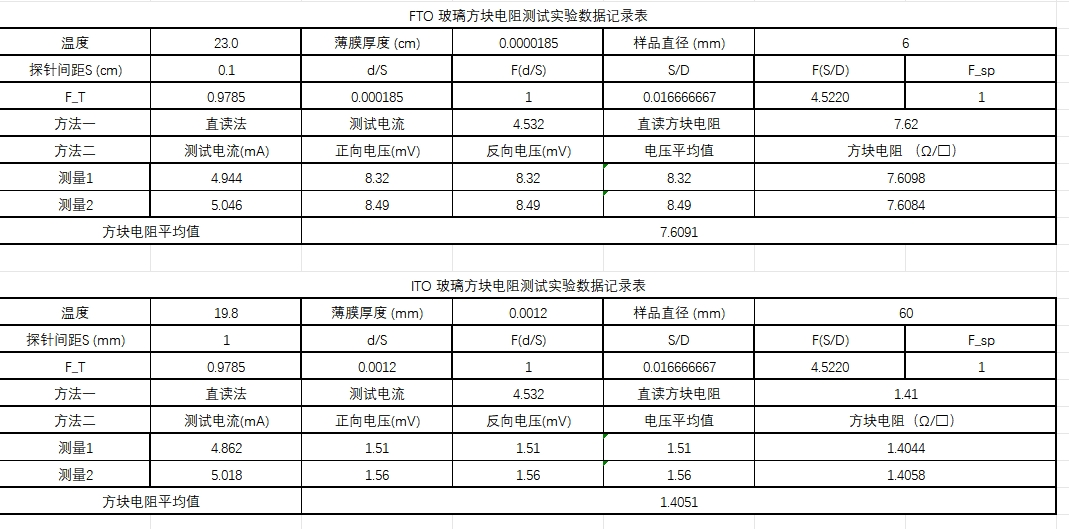
\includegraphics[width=80mm]{2.png}}
        \end{floatrow}
    
    \end{figure}

\section*{【实验数据处理与结果分析】}
    \subsection*{实验数据处理}

按照前文给出的公式,在excel表中计算得到了如上数据。其中,按照当天气温(23.0摄氏度)给出了$F_{t}$

对于表格二的数据,其余数据均按照线性插值查表得到,即$F_{sp} $=1,F(d/S)=0.9993,F(S/D)=4.5254
得出数据在表格中均有填写,不再赘述。

    \subsection*{实验二测量 p 型单晶硅片(薄样品)的电阻率的不确定度分析}
    已知数字电压表的测试量程为 0.2mV$\sim$50mV,分辨率优于
    ±0.05\%。在 1mA 电流档,恒流源最大允许误差为±0.02 mA;在 10mA 电流档,恒流源最大
    允许误差为±0.1 mA。硅片厚度测量结果的相对不确定为±0.2\%。探针间距修正因子 $F_{sp}$、样品
    厚度修正因子 F(d/S)和直径修正因子 F(S/D)引入的不确定度可以忽略。假定矩形分布来评估
    仪器精度引入的不确定度。计算硅片电阻率测量结果的相对不确定度。假设包含因子 k=2,
    给出扩展不确定度。

    对于第一次测量结果:
\begin{equation*}
    \rho = \frac{V}{I} \cdot d \cdot F_{sp} \cdot F(d/S) \cdot F(S/D)
\end{equation*}
    V的A类不确定度:V取了两次电压平均值计算。平均值为69.570 mv,由此计算其标准差,即为电压的A类不确定度
    \begin{equation*}
        u_a =(\frac{\Sigma (x_i-\bar{x})^2}{n(n-1)})^{1/2}
    \end{equation*}
    得到$u_a$=0.14,此处乘以修正因子$t_p$可以得到修正后的不确定度。如下表,
    \begin{center}
        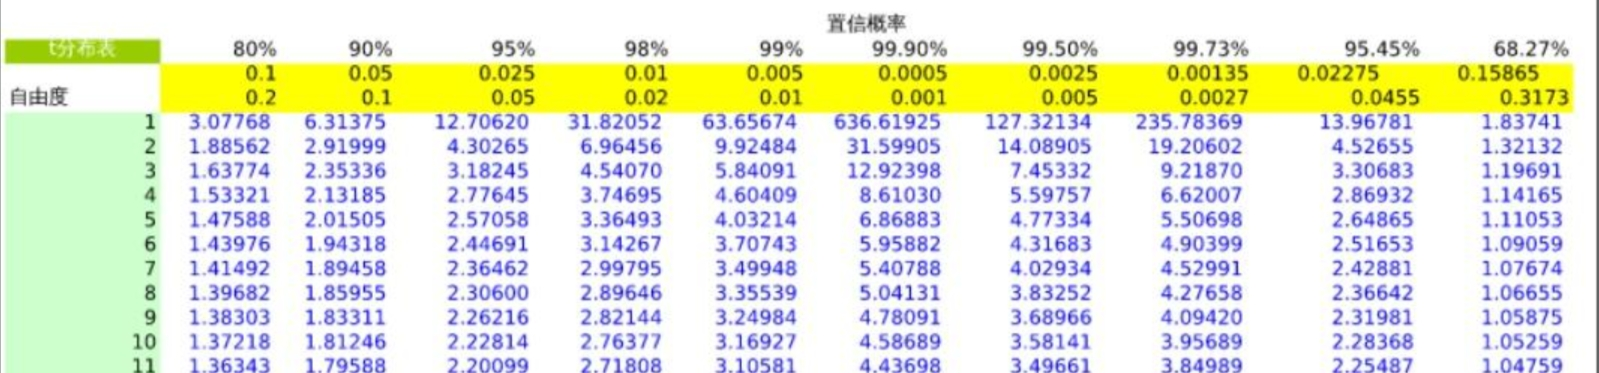
\includegraphics[width=400pt]{3.png}
    \end{center}
    $u_a$=0.18498 mV

    V的B类不确定度:电压表精度为±0.025mV,
    \begin{equation*}
        u_b = k_p \cdot \Delta / C
    \end{equation*}
    其中,C 取$3^(1/2)$,$\Delta $取最大精度,$k_p$ 取1

    $u_b$=0.014434 mV
    
    同理其他量的不确定度为:

    $I_a$=0,$I_b$=0.01155 mA,$d_b=0.002*0.04=0.00008cm$

    合成不确定度:
    $u^2={u_a}^{2} + {u_b}^{2}$,有

    $u=0.185547 mV ,I=0.01155mA,d=0.00008cm$

    接下来,求合成标准不确定度:
    \begin{center}
        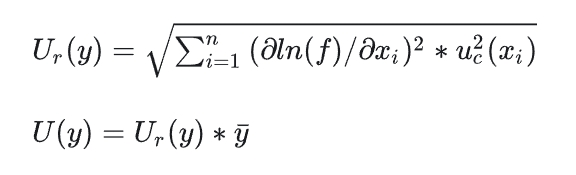
\includegraphics[width=200pt]{4.png}
    \end{center}

    所以${U_r}^2= \frac{u^2}{{U}^2} + \frac{i^2}{{I}^2} + \frac{d^2}{{D}^2}$
    
    相对误差$U_r=0.0002989$,$U_{r2}=0.0208 $

    $\Delta N=k \cdot U_{r2}| =2 \cdot U_r=0.0416$,(k=2)

    即$\rho $的拓展不确定度为0.0416,$\rho =69.570 \pm 0.0416 \Omega \cdot cm$

    可以看出此处的拓展不确定度比较小,说明,实验的操作得当。

\subsection*{结果分析}
        \begin{enumerate}
            \item 表一可知,电阻率平均值为1.6910 $ \Omega \cdot cm$,电阻率$ \rho $不均匀度为0.9449\%,
            数值上,电阻率偏差小,不均匀度小,且电阻率在样品的电阻率范围内,数据做得相对不错。
            \item 表二可知,直读法和计算得出的数值很接近,这也说明了操作上没有出现很大的问题。测量本身的不确定度就相对高。
            \item 表三、四、五可知直读法和计算得出的数值很接近,FTO 玻璃方块电阻测试实验的数据差值远小于0.1\%左右,扩散片方块电阻测试实验数据差值在0.1\%左右,
            ITO 玻璃方块电阻测试实验数据数据差距在0.05\%左右,这更说明了,我们使用的方法以及操作方法没有问题。					

        \end{enumerate}
\section*{【思考题】}
\begin{center}
    一、电阻率和方块电阻的测量结果的误差来源有哪些?应如何避免? 
\end{center}
 

\begin{enumerate}
    \item 在测量过程中,由于实验仪器的显示位数,测量精度等方面影响,测量值有偶然误差,可以通过多次测量取平均值在一定程度上可以减小这种误差。
    \item 实验所用的公式是由理想模型推导,实际测量的样品可能需要一定程度上的修正,故引入了直径、厚度修正因子。
    \item 样品本身制样的问题。样品本身在制样过程中无法做到完全均匀,完全满足我们计算理论公式的时候使用的假设,会导致误差增大。
    \item 在读数和计算过程中带来的误差,四舍五入等操作会影响测量结果,在计算过程中优先多保留几位小数计算可以减小这种误差。
    \item 实验的仪器精度不够,实验仪器精度不够的话,会导致误差,更换更好的仪器可以减小误差。
    \item 外界环境带来的误差,例如温度,湿度,同时环境温度和湿度地测量不够准确。在实验中,我们根据环境温度采用了温度修正因子,同时,湿度对于本实验可能也有影响,可以考虑其影响。
    \item 操作失误或者计算错误也会带来很大的不确定度,如在移动样品时未穿戴手套,故应当穿戴手套并使用镊子完成样品的更换等工作,规范操作,认真计算即可。

\end{enumerate}

\begin{center}
    二、影响测量结果准确性的外界因素有哪些?应如何避免?
\end{center}

\begin{enumerate}
    \item 环境因素的影响。例如温度、湿度,一方面需要引入温度、湿度的修正因子,另一方面我们需要更精准地测量样本周边的环境温度和湿度,另一方面需要更精准的不需要用插值法求得的修正值。
    \item 外界环境污染的影响。外界可能在样品表面产生包括灰尘,油脂等污染物质,同时实验所用的样品并没有很好的保护特别是在经由多次实验后可能被污染,进而影响材料电阻率的测量。因而在进行试验时要穿戴手套,用镊子,并可以考虑用合适的试剂适时地对样品进行清洁保护。
    \item 实验仪器精度问题。更换更好的仪器,或者使用误差更小的方法进行测量。
    \item 样品本身制样的问题。样品本身在制样过程中无法做到完全均匀,完全满足我们计算理论公式的时候使用的假设,会影响测量结果。
\end{enumerate}
\end{document}